\section{Theory}
\label{sec:Theorie}

The molar heat capacity is defined by 
\begin{equation}
    C = \frac{\Delta Q}{\Delta T}.
\end{equation}

It describes the proportion between the amount of heat $Q$ to raise the tempreture $T$ of a material. 
Regarding the first law of thermodynamics
\begin{equation}
    \symup{d}Q = \symup{d}U+p\symup{d}V,
\end{equation}
the variation of heat is dependend of the pressure $p$ and the volume $V$.
For experimental purposes it is beneficial to keep the pressure or the volume constant.
The difference between these two cases is given by
\begin{equation}
    C_p - C_V = T V \alpha_V^2 B.
\end{equation}
$T$ is the temperature, $V$ the volume, $\alpha_V$ the expansion coefficient and $B$ the bulk modulus.
So this difference depends on properties of the respective material and the state of aggregation. 
Because of the small expansion coefficients of cristalls, the difference between the two heat capacities is neglectable.
For experimental practicability, often the heat capacity by constant pressure is used.


\subsection{Dulong-Petit}
In the classical theory the heat capacity is constant and only depends on the number of degrees of freedom $f$ of the system:
\begin{equation}
    C = \frac{f}{2} R.
\end{equation} 
For a three dimensional cristall, every atom has three possible directions to oscillate. 
In average the atoms have the same kinetic and potential engergy of 
\begin{equation}
    E = \frac{1}{2}k_B T,
\end{equation}
with $k_B$ the Boltzman constant.
So every atom has six degrees of freedom. 
Eventually the heat capacity results to
\begin{equation}
    C = 3 R,
\end{equation}
where $R$ is the gas constant.
This result only holds for high temperatures. 
In contradiction experimental messurements by low temperatures are showing a $T^3$-proportionality.
This law is only explainable with quantum effects.

\subsection{Einstein model}

To get a more precize describtion of the thermic behavior of cristalls, the model has to take quantum mechanics into account. 
Now the engergy of the osscilations are quantized.
The Einstein model assumes a constant frequency $\omega = \omega_E$ for all atoms.
This assumption is good to approximate a typical dispersionrelation for optical branches, which is shown in figure \ref{fig:disperion}. 
The heat capacity results to 
\begin{equation}
    C_V^E = 3 N k_B\left(\frac{\Theta_E}{T}\right)^2\frac{e^{\frac{\Theta_E}{T}}}{\left(e^\frac{\Theta_E}{T}-1\right)^2},
\end{equation}
where $N$ is the number of particles, $k_B$ is the Boltzman constant and $\Theta=\frac{\hbar \omega_E}{k_B}$ the Einstein temperature.
For high temperatures this expression tends to the law of Dulong Petit.
In the low temperature area the experimental result diverges from the theoretic predictions of this model.
This is explainable with the assumption of constant frequencies, because for low temperatures most states not in the optical branches but in the accustical branches.
To approximate these branches it needs a linear disperionrelation.

\begin{figure}
    \centering 
    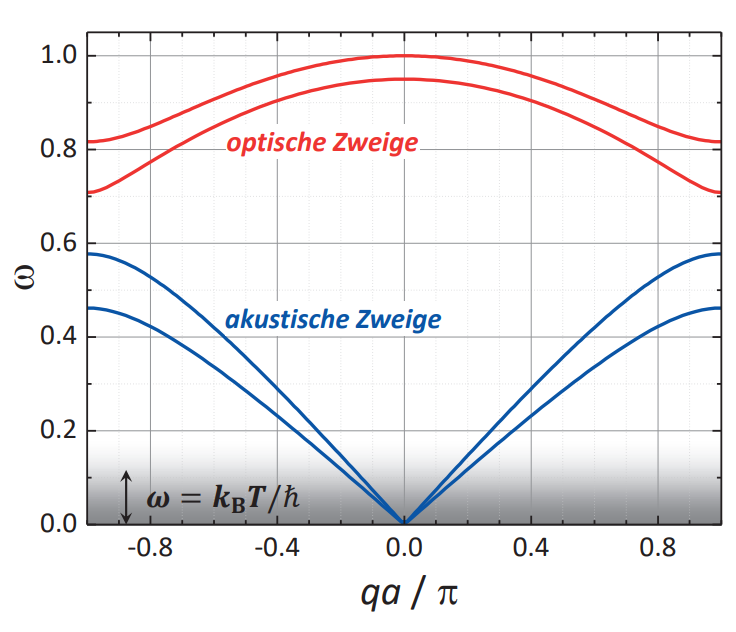
\includegraphics[width=.8\textwidth]{bilder/Disperion.png}
    \caption{Typical disperion relations of an one atomic cristall. \cite[S. 223]{gross2012festkoerperphysik}}
    \label{fig:disperion}
\end{figure}


\subsection{Debey model}
Unlike the Einstein model the Debey model assumes a linear dispersionrelation with an maximal value $\omega_D$, called the Debey frequency.
The Debey frequency is defined by
\begin{equation}
    \label{eq:Debey}
    \int_0^{\omega_D}Z(\omega) \symup{d}\omega = 3 N_L,
\end{equation}
with 
\begin{equation}
    Z(\omega) = \frac{L^3}{2\pi^2}\omega^2\left(\frac{1}{v_\text{long}^3}+\frac{2}{v_\text{trans}^3}\right)
\end{equation} 
as the spectral frequency distribution of the oscillators and $N_L$ as the Loschmidt constant.
$v_\text{long}$ and $v_\text{trans}$ are the respective phase velocities of the logitudinal- and transversal oscillations.
To calculate $\omega_D$, the equation \eqref{eq:Debey} can be transformed into
\begin{equation}
    \label{eq:omega}
    \omega_D = \left[\frac{18\pi^2N_L}{L^3}\left(\frac{1}{v_\text{long}^3}+\frac{2}{v_\text{trans}^3}\right)^{-1}\right]^\frac{1}{3}.
\end{equation}
In this model the heat capacity is given by the equation:
\begin{align}
    \label{eq:cvv}
    C_V^E &= 9Nk_B\left(\frac{T}{\Theta_D}\right)^3 \int_0^{\frac{\Theta_D}{T}}\frac{x^4e^x}{\left(e^x-1\right)^2} \symup{d}x \\
    & =
    \begin{cases}
    \frac{12\pi^4}{5}Nk_B\left(\frac{T}{\Theta_D}\right)^3 , & T \gg \Theta_D \\
    3Nk_B , & T \ll \Theta_D \label{eq:cases}
    \end{cases}
\end{align}

$\Theta_D=\frac{\hbar \omega_D}{k_B}$ is the Debey temperature and can be used to estimate the heat capacity for higher or lower temperatures.
As equation \eqref{eq:cases} suggests the messured $T^3$-proportionality is given for low temperatures. 
Furthermore the limit of high temperatures matches the Dulong Petit law.





%In knapper Form sind die physikalischen Grundlagen des Versuches, des Messverfahrens, sowie sämtliche für die Auswertung erforderlichen Gleichungen darzustellen. (Keine Herleitung)

%(eventuell die Aufgaben)

%Der Versuchsaufbau: Beschreibung des Versuchs und der Funktionsweise (mit Skizze/Bild/Foto)
